\chapter{Nasazení}
 Produkční server běží v~rámci školní infrastruktury. Pro úspěšné nasazení stačí vzít zdrojové soubory, nastavit soubor \texttt{.env} podle souboru \texttt{.env.example} a~spustit příkaz \texttt{docker compose up -d} jak pro serverovou, tak pro klientskou aplikaci. Po nasazení systému se doporučuje pro každý scraper spustit příkaz \texttt{ssh <username>@perun.fit.vutbr.cz "docker exec -d <scraper container id> nohup scrapy crawl <scraper name> \&"}. \\Jednotlivé scrapery mohou běžet paralelně, ale je vhodné rozložit scrapery pro více archivů, aby nedocházelo ke zbytečnému přetěžování konkrétního archivního systému. O~následnou aktualizaci dat se stará úloha cron, která periodicky stahuje datové sady a~aktualizuje záznamy v~databázi.


\begin{figure}[htbp]
\centering
    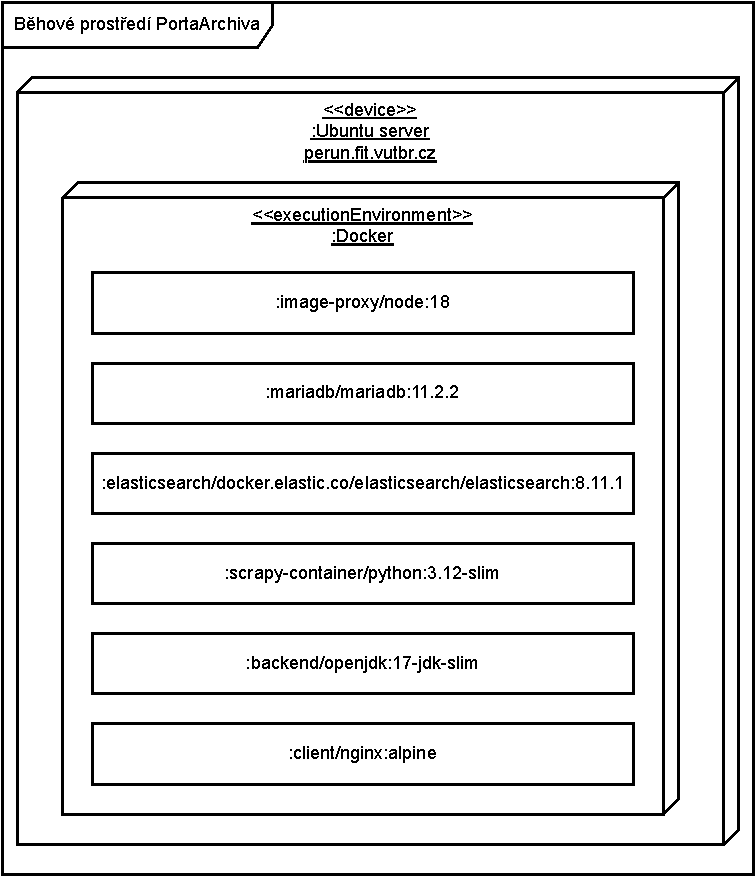
\includegraphics[scale=1]{obrazky-figures/deployment/deployment_diagram.pdf}
    \caption{Diagram nasazení}
\end{figure}